\chapter{Background}
The biologist Carl Woese suggested that “Organisms are resilient patterns in a turbulent flow—patterns in an energy flow” \parencite{Woese}. If this somewhat captures life, then the formation and maintenance of patterns are essential. On the sub-cellular level, an important component conferring structure and organization is the cytoskeleton. The cytoskeleton is a complex, dynamic network of protein filaments which can be found in the cytoplasm of all cells, including bacteria and archaea. Eukaryotes employ three different types of filaments: microtubules, actin filaments and intermediate filaments. These filaments interact interact with a plethora of other biopolymers in the cell, allowing the cytoskeleton to fulfill vital functions in a diverse set of domains, such as locomotion of the cell, maintaining structural integrity, chromosome segregation and cytokinesis during mitosis and the transport of cargoes within the cell. The cytoskeleton confers structure to the cell, but what confers structure to the cytoskeleton itself? While some of the patterning stems from interactions with other large entities, such as the cell membrane, the organization of the cytoskeleton partly emerges from the collective behavior of the involved cytoskeletal polymers. In other words, the cytoskeleton and its associates are known to display self-organization \parencite{Karsenti2008}. This work aims to expand our understanding of how, and to which extent, cytoskeletal polymers interact to give rise to supramolecular patterning. \par
To minimize the number of factors which could possibly give rise to patterns such to reveal underlying molecular mechanisms, we followed a bottom-up approach, where we sought to reconstitute cytoskeletal features \textit{in-vitro} with a minimum number of components. We focused on microtubules, where we were interested in two cytoskeletal systems of which they are prominent members: (1) Axonal microtubule arrays and (2) the mitotic spindle. These two systems are very different, which is reflected in the different behavior of microtubules within them. Thus, this thesis contains two parts, each dedicated to one of these systems. Each of them is introduced below, together with the microtubule-associated proteins explored in the respective experiments (see \autoref{sec:neuron} for axonal microtubule arrays and \autoref{sec:spindle} for the mitotic spindle). As in both systems, microtubules are an integral part of the experimental setup, I in \autoref{sec:microtubules} offer an introduction to them. I also give a brief primer on the biological, chemical and physical characteristics of proteins in general (\autoref{sec:proteins}), as well as on the most prominent methods used in the course of this work \pref{sec:methods_intro}{}.

\section{Foundations}
\subsection{Proteins}
\label{sec:proteins}
TODO: mention intrinsically disordered proteins

\subsection{Microtubules}
\label{sec:microtubules}
Microbules are long hollow tubes present in all eukariotic cells. They play important roles in a number of processes, including in cell division, intracellular transport, and cell motility \parencite{Akhmanova2022}.

\subsubsection{Subunits}
\label{sec:tubulin}
Microtubules are comprised of heterodimers of the protein \textit{tubulin}. In cells, tubulin exists almost exclusively as the $\alpha\beta$-tubulin heterodimer. $\alpha$- and $\beta$-tubulin are conserved throughout eukaryotes, sharing over 40\% sequence identity with nearly the same secondary and tertiary structures \parencite{DOWNING199816}. Each tubulin monomer is a globular protein and consists of three closely interacting domains: an N-terminal nucleotide-binding domain, an intermediate domain, and a carboxy-terminal (C-terminal) helical region \parencite{ALUSHIN20141117}. The disordered, negatively charged C-terminal tails of tubulin protrude outwards from the microtubule surface.\par

As is the case with many other proteins, tubulins express in different isoforms, arising from the expression of alternative tubulin-encoding genes. In humans, $\alpha$- and $\beta$-tubulin are encoded in 9 genes each \pcite{Janke2020}. Many, but not all, of these subtypes are highly conserved across species \pcite{Janke2020}, in other words, they are almost identical. Tubulins further can be modulated by post-translational modifications, thus providing an additional level of microtubule regulation \parencite{Janke2014}. Modification of the C-terminal region in particular has been found to affect microtubule properties and their interactions with other proteins \parencite{Janke2020}. 

\begin{figure}[h!tb]
	\centering
	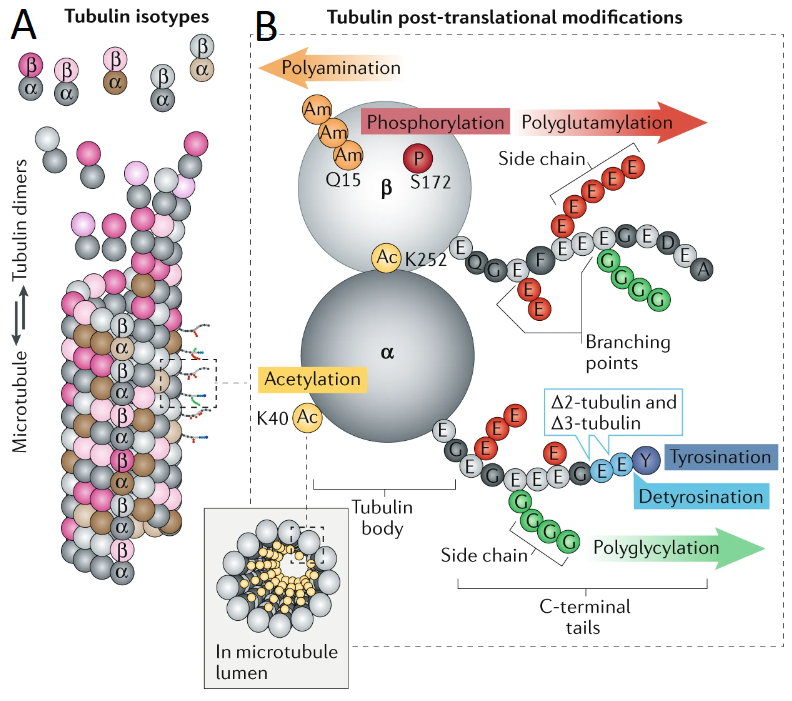
\includegraphics[width=0.6\linewidth]{Figures/tubcode.png}
	\caption[Introduction to tubulin.]{\textbf{Introduction to tubulin.}
	(A) Microtubules are constituted by $\alpha$- and $\beta$-tubulin, which in humans are expressed in different isoforms. (B) $\alpha$- and $\beta$-tubulin can undergo various types of post-translational modifications. This includes additions of groups, mainly to the C-terminal of either tubulin, but also other sites, e.g., the acetylation of a $\alpha$-tubulin residue pointing toward the inside of the microtubule (the lumen). It also includes detyrosination, which is the removal of a tyrosine from the $\alpha$-tubulin C-terminal. Taken from \cite{Janke2020}.
		}\label{tubcode}
\end{figure}

\subsubsection{Structure}
The microtubule lattice can be described as a lateral association of so-called protofilaments, which are linear strands of $\alpha$- and $\beta$-tubulin heterodimers (\autoref{MTintro}A). Their arrangement in a ring leads to the cylindrical structure of microtubules with an outer diameter of approximately 25 nm and an inner diameter of 17 nm (\autoref{MTintro}B, \pcite{Hawkins2010}). The hollow tube architecture of microtubules allows for the high persistence length of microtubules, which is in the low millimeter range \parencite{Hawkins2010}. This high persistence length allows MTs to stretch over distances comparable to the size of a whole cell. Owing to the uniform orientation of the tubulin dimers, microtubules are directional polymers, with the $\beta$-subunits pointing to one end (called ‘plus end’) and the $\alpha$-subunits pointing to the opposite end (called ‘minus end’). \par

In cells, microtubules usually have 13 protofilaments, however, in some cell types, microtubules with a different number of protofilaments have been observed, with observed numbers ranging from 11 to 15. For example, the nerve cords of nematodes harbour MTs with 11 protofilaments, and 15-protofilament microtubules have been found in various animal cells implicated in mechanosensation \parencite{Chaaban2017}. Meanwhile, microtubules polymerized \textit{in vitro} feature between 9 and 16 protofilaments \parencite{Chaaban2017}. The number of protofilaments appears to be partially determined by the isotype of the involved tubulin dimers \parencite{Ti2018}. \textit{In vitro}, the number of protofilaments also depends on whether and how the microtubules have been stabilized \aref{sec:stabilization}{}. This flexibility in terms of protofilament number allows for lattice defects to occur where the number of protofilaments may differ in different parts of a given microtubule \pcite{Chretien}. It is also worth noting that depending on the number of protofilaments, the protofilaments in a given microtubule align differently: In the 13-protofilament variant, microtubules have a helical pitch of 1.5 dimers, i.e., their structure repeats every 1.5 dimers. Here, protofilaments are in an arrangement where tubulin subunits laterally associate with the opposite type (i.e., $\alpha$- with $\beta$-tubulin), except at the seam, where tubulins of the same type associate (\autoref{MTintro}B). A different number of protofilaments typically results in a different pitch, and in some instances in microtubules without a seam \pcite{Hawkins2010}. Finally, a different number of protofilaments typically results in a structure where protofilaments no longer are straight but curl around the microtubule \parencite{Chaaban2017}.

\subsubsection{Polymerization}
\label{sec:instability}
Microtubules grow in every eukaryotic cell and can also be polymerized \textit{in vitro}, i.e., in assays outside of cells given an adequate experimental buffer. Notably, the spontaneous assembly of microtubules, i.e., spontaneous \textit{microtubule nucleation}, is kinetically unfavorable because the intermediate tubulin structures required for forming a full ring are not very stable \parencite{Akhmanova2022}. Spontaneous nucleation thus can occur only at high concentrations of free tubulin \parencite{Fygenson1994}. In a more kinetically favorable mechanism, the \textit{de novo} assembly of microtubules is partly directed by designated $\gamma$-tubulin nucleation complexes, which provide templates for the outgrowth of new microtubules \parencite{Akhmanova2022}. These nucleation complexes can be found in microtubule-organizing centers such as the centrosome of the spindle (\autoref{sec:spindle}), and in some cases also along pre-existing microtubules \parencite{Akhmanova2022, Janson2007}. Another means by which the cell can multiply the number of microtubules is by severing existing microtubules (\cite{Vemu2018}, see \autoref{sec:katanin_intro}). Notably, the fact that spontaneous nucleation is kinetically unfavorable gives the cell a high degree of control over the number and distribution of microtubules over time and space. \par

In spite of their high persistence length, microtubules are no static structures. Instead, their plus ends are stochastically switching between phases of growth and shrinkage \parencite{Janosi2002}. This property is termed \textit{dynamic instability}. According to the widely accepted and GTP cap model of microtubule instability \pcite{Gudimchuk2021}, microtubule dynamic instability stems from the existence of two conformationally distinct populations of tubulin dimers: GTP-tubulin and GDP-tubulin, having GTP respectively GDP bound to their $\beta$-tubulin. Mostly, it is free GTP-tubulin that adds to the lattice of a polymerizing microtubule. Shortly after polymerization, the $\beta$-tubulin hydrolyzes its GTP, resulting in conformational changes which result in mechanical tension. GTP-hydrolysis of a lattice-incorporated tubulin has no immediate consequences for the microtubule as a whole. However, if GTP-hydrolysis occurs at a microtubule end, the higher degree of freedom allows for conformational relaxation and eventual removal of GDP-tubulin from the microtubule end. This conformational relaxation typically takes the form of a curving of the protofilament, breaking lateral bonds with neighbouring protofilaments and thereby further destabilizing the microtubule end. Thus, if a microtubule loses too many GTP-tubulins at its plus end, i.e., if it loses its GTP cap, it switches to a regime of quick depolymerization where most protofilaments are curved outwards (\autoref{MTintro}C). While the GTP cap model of dynamic instability is experimentally strongly supported, there is less clarity on why exactly GTP-tubulin lattices are more stable than GDP-lattices, and multiple, non-mutually-exclusive models exist \pcite{Gudimchuk2021}. In one model, GTP tubulin dimers are straighter than GDP tubulin dimers already in their relaxed state, facilitating their lattice incorporation. In another model, GTP tubulin might more readily change into a straight conformation than GDP tubulin. A third model proposes that GTP hydrolisis introduces relevant conformational changes at the interface between the adjacent dimers of a given protofilament. There certainly is evidence that GTP hydrolisis introduces changes at these interfaces \pcite{Alushin2014}.\par

A change from continued polymerization to rapid depolymerization is called a \textit{catastrophe} event. A reversal from depolymerization to polymerization can also occur and is called a \textit{rescue} event. In the absence of rescue-promoting microtubule-associated proteins \pref{sec:MAPs}{}, rescues are currently hypothesized to occur mainly at positions where GTP islands have formed within the otherwise GDP-dominated microtubule lattice. This hypotehsis is supported by \textit{in vitro} experiments showing rescues to coincide with GTP islands \pcite{Aumeier2016}. These islands had further been shown to be the result of microtubule self-repair, i.e., instances where free GTP-tubulin was incorporated into a damaged part of the microtubule \pcite{Aumeier2016}. Recently, microtubule self-repair and GTP islands have also been observed \textit{in vivo} \pcite{Gazzola2023}.\par

As a final note, microtubule minus ends \textit{in vivo} have not been observed to elongate, i.e., microtubule polymerization happens exclusively at the plus end \parencite{dammer}. \textit{In vitro}, minus ends can also exhibit polymerization, yet the plus end nonetheless polymerizes more quickly and is generally more dynamic \parencite{Howard2003}. 

\begin{figure}[h!tb]
\centering
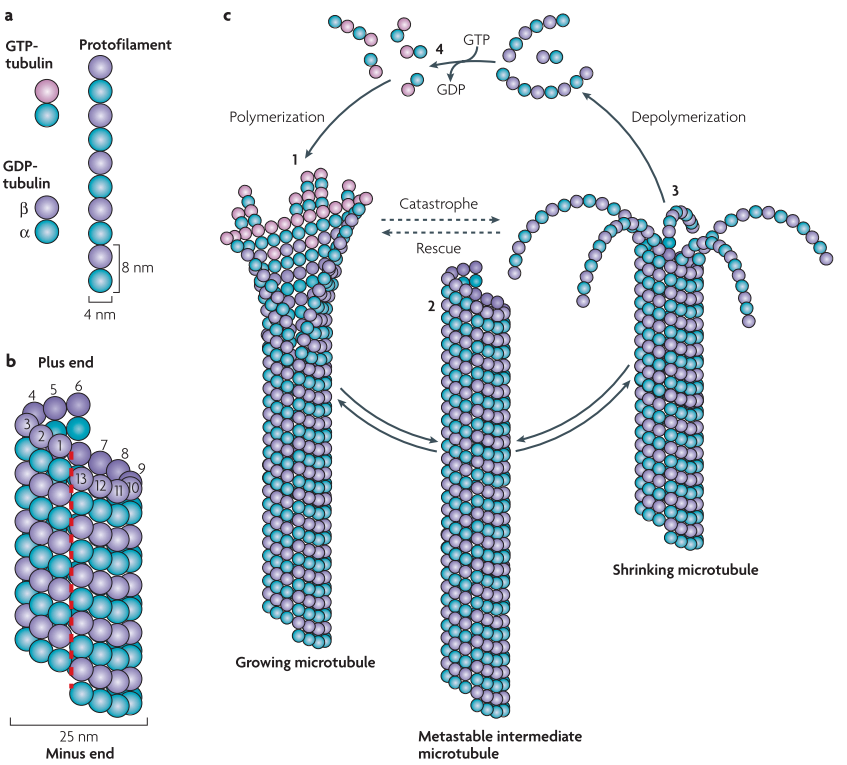
\includegraphics[width=\linewidth]{Figures/MTintro.png}
\caption[Introduction to microtubules.]{\textbf{Introduction to microtubules.}
(A) Microtubules consist of $\alpha\beta$ heterodimers. While $\alpha$-tubulin normally retains its GTP, the GTP molecule of $\beta$-tubulin can be both hydrolyzed and exchanged for ADP. (B) \textit{In vivo}, microtubules are composed of 13 protofilaments. Since the \SI{12}{\nm} helical pitch does not equal the dimer length, a lattice seam occurs. (C) Due to the GTP-hydrolysis of incorporated $\beta$-tubulin, microtubule ends undergo a permanent cycle of growth (1) and shrinkage (3), closed by the exchange of GDP for GTP for the disassembly products (4). This cycle can briefly come to a halt during a less prevalent metastable state (2), from which microtubules can switch either to growth or to shrinkage. All sketches adapted from \cite{Akhmanova2008}.
	}\label{MTintro}
\end{figure}

\FloatBarrier

\subsubsection{Microtubule-associated proteins}
\label{sec:MAPs}
The vast functional diversity of microtubules is enabled by their interactions with microtubule-associated proteins (MAPs). \cite{BODAKUNTLA2019804} categorize MAPs into different groups depending on their mode of action, namely i) molecular motors generating movement along microtubules, ii) enzymes destabilizing the microtubule lattice, iii) MAPs promoting microtubule nucleation, iv) microtubule-end binding proteins and v) structural MAPs controlling microtubule polymerization, stabilization and assembly into microtubule bundles. One MAP may belong to several of these groups, for instance, the molecular motor Kip3 is known to also cause microtubule polymerization \parencite{Gardner2011a}. In the course of my work, I have worked with four different MAPs as introduced further below, namely tau \pref{sec:tau_intro}{}, kip3 \pref{sec:kip3_intro}{}, katanin \pref{sec:katanin_intro}{}, and Ase1 \pref{sec:Ase1_intro}{}. 

\subsection{Employed technologies}
\label{sec:methods_intro}
Below a primer on some of the main technologies which enabled the work performed for this thesis.

\subsubsection{In-vitro stabilization of microtubules}
\label{sec:stabilization}
For in-vitro experiments, it often is desirable to stabilize microtubules such that they remain polymerized even in the absence of GTP and/or free tubulin, in other words, to prevent microtubule instability. There are two popular methods, which I had both employed during my work:
\begin{itemize}
	\item \textbf{Stabilization via GMPCPP.} GMPCPP is a non-hydrolyzable analog of GTP that binds to the GTP-binding site of tubulin. By mimicking GTP, GMPCPP stabilizes the microtubule lattice, without any hydrolisis occurring which would normally induce lattice instability. This stabilization allows microtubules to remain polymerized even in the absence of free tubulin, GTP, or GMPCPP \parencite{Hyman1992}.
	\item \textbf{Stabilization via paclitaxel}. Paclitaxel, also known as taxol, does not directly interfere with the GTP cycle of tubulin but rather binds along the microtubule. This binding enhances microtubule stability, even under conditions that would normally induce shrinkage, such as low tubulin concentrations \parencite{SCHIFF1979}. Notably, paclitaxel is not tightly bound to microtubules \pcite{Diaz98}, and thus paclitaxel-stabilized microtubules need to be stored in buffer solutions containing paclitaxel.
\end{itemize}
It is worth noting that the choice of stabilization impacts the mechanical properties of microtubules. For example, paclitaxel-stabilized microtubules tend to have fewer protofilaments than GMPCPP-stabilized microtubules. Paclitaxel-stabilized microtubules feature a wide variability in their protofilament number, with the most common number being 12 protofilaments, while GMPCPP-stabilized microtubules typically feature 14 protofilaments \pcite{Andreu1992, Meurer}. Also, GMPCPP-stabilized microtubules have been measured to have twice the flexural rigidity of paclitaxel-stabilized microtubules \pcite{Mickey1995}.

\subsubsection{Green fluorescent protein}
Green fluorescent protein (GFP) was discovered around 60 years ago in the jellyfish Aequorea victoria \pcite{shimomura2005discovery}. 

\subsubsection{Total internal reflection (TIRF) microscopy}
The main experimental method employed during the course of this work was total internal reflection fluorescence (TIRF) microscopy. TIRF microscopy takes advantage of the physical phenomenon of total internal reflection, whereas light is fully reflected from a surface, yet a so-called evanescent field emanates beyond the surface of reflection, decaying exponentially in intensity. Because the evanescent field does not propagate, this phenomenon allows to selectively illuminate fluorophores near the glass/water surface, in our case the immobilized microtubules and their associated MAPs. By avoiding to excite fluorophores further away from the immobilized microtubules, background fluorescence can be reduced, as mainly the fluorophores of interest are excited. This is crucial for assays with a large number of labeled proteins in solution. 

\subsubsection{Interference reflection microscopy (IRM)}
For a few experiments (as indicated in methods section) we had employed interference reflection microscopy (IRM). In contrast to fluorescence-based microscopy methods, IRM allows for label-free imaging of biological samples. In the IRM setup, light from the light source passes through the aperture diaphragm and the field diaphragm, which regulate the amount of light reaching the camera. The 50/50 mirror then divides the light into two beams: one transmitted and one reflected, each with half the intensity of the original beam. The reflected beam is directed toward the objective, reflects off the sample, and then travels back through another 50/50 mirror and the tube lens to the camera. The resulting image is determined by the interference of reflections at the glass/water and water/sample interfaces. These reflections are influenced by differences in refractive indices — greater differences result in higher intensity of the reflected light beam \parencite{barr2009interference}. IRM thus requires particles large enough to generate noticable shifts in the phase of the reflected light. Due to the relatively large size of microtubules, IRM can be used to visualize them, with the advantage of requiring relatively few changes to typical microscope setups compared to more advanced techniques such as interferometric scattering (iSCAT) microscopy \parencite{Mahamdeh2018}.

\subsubsection{Fluorescence recovery after photobleaching (FRAP)}
\label{sec:FRAP}
We for a few experiments also employed fluorescence recovery after photobleaching (FRAP) to investigate the binding kinetics of microtubule-associated proteins (MAPs). In the FRAP setup, a focused laser, in our case using the TIRF setup, is used to photobleach fluorescently-labelled molecules within a given region, creating a dark spot. The recovery of fluorescence in this region is then monitored over time as unbleached molecules diffuse into or associate with the bleached microtubule area, while bleached molecules dissociate or move away \parencite{axelrod1976mobility}. FRAP was a relevant for us due to its ability to provide insights into the unbinding rate $k_{off}$ of a given microtubule-associated protein. If the binding sites on a microtubule for a given MAP are covered such that an equilibrium exists (i.e. no net binding or unbinding of MAPs occurs), after bleaching all of the MAPs on that microtubule, the rate of recovery depends only on $k_{off}$, assuming that the fluorescent MAPs in solution were not significantly depleted by the photobleaching \parencite{bulinski2001rapid}, which in our case is true due to our employment of TIRF. Specifically, to determine $k_{off}$, one can fit the following function to the signal $I(t)$ measured experimentally by imaging the region over time (taking care to not signficantly bleach the sample due to this imaging): $I(t)=1-e^{-k_{off}t}$ \parencite{bulinski2001rapid}.

\section{Microtubule systems}
Microtubules behave differently and fulfill different functions depending on the cellular context they are in. The two systems where I with this thesis aim to contribute understanding to are axonal microtubule systems (with a focus on tau, katanin, and kinesin-8) and the mitotic spindle (with a focus on Ase1).

\subsection{Axonal microtubule arrays}
\label{sec:neuron}
The complex development and functionality of the nervous system rely heavily on microtubule-related processes, as microtubules play key roles in guiding cellular organization and intracellular transport \parencite{Kapitein2015}. Prominently, neurons develop two types of cytoplasmic protrusions: (i) Axons (also called nerve fibers) and (ii) dendrites. A typical neuron has one axon, which can reach to distant parts within the animal's body, and multiple dendrites, which are shorter, and connected to axons via synapses. While axons primarily contain long, stable microtubules, dendrites harbor shorter, more dynamic microtubules \parencite{Tas2017}. To understand their cellular context, it is instructive to introduce axonal microtubule arrays vis-a-vis dendritic microtubule arrays.\par

Regarding intracellular transport, microtubules prominently serve as highways for molecular motors, most prominently kinesins, but also dyneins which are minus-end directed motors \parencite{Kapitein2015}. Efficient directional transport is especially crucial in neurons, given that dendrites and especially axons grow to macroscopic lengths. It is thus not surprising that within axons, microtubules bundle and point toward the same direction, namely with their plus ends away from the cell body (the soma) toward the distal end of the axon \parencite{Tas2017}. Such an alignment lends itself to efficient transport of cargo between these distant parts of the cell, as a given motor cannot accidentally switch to an antiparallely aligned microtubule and travel in the opposite direction than previously. At the same time, within mammalian dendrites, there are both inward- and outwardpointing microtubules in equal parts \parencite{Tas2017}. Here, sufficiently effective transport is achieved by bundling microtubules such that a given bundle in a given dendrite predominantly comprises microtubules of the same orientation \parencite{Tas2017}. Notably, and puzzingly, despite the existence of plus-end-outward microtubules in dendrites, many plus-end directed motors, including kinesin-8, only enter the axon \parencite{Lipka2016}.\par

Regarding the guiding of cellular organization, the remodeling of microtubule arrays plays a central role in cell migration as well as the development of axons, dendrites, and synaptic connections \parencite{Kapitein2015}. For example, some molecular motors transport signaling factors or can even have non-motor signaling functions themselves, and as such the positioning of the microtubules becomes a determinant of developments within the cell \parencite{Hirokawa2010}. Microtubules and microtubule motors are also involved in generating mechanical forces that drive cellular processes. For instance, dynein motors, by sliding axonal microtubules against each other, can push microtubules into growth regions of the axon, thereby in their interplay with opposing kinesin motors co-determining the direction of axonal growth \parencite{Kahn2016}. Notably, post-translational modifications of tubulin (see \autoref{sec:tubulin}) play an essential role in fine-tuning MT dynamics and stability. Tubulin acetylation, for example, is associated with stable microtubules, which can be found e.g. in the axonal shaft but also in dendrites \parencite{Tas2017}. Dynamic (or "labile") microtubules, which undergo frequent cycles of growth and shrinkage, comprise less acetylated tubulin, and can be found in dendrites and at the tips of growing axons, where active remodeling is necessary \parencite{Baas2016, Tas2017}. In this context, it is also notable that Katanin levels in neurons are highest during developmental stages where a high dynamicity is required, and both depleting and overexpressing the p60 subunit have been shown to result in impaired neuronal development \parencite{Karabay2004}.\par

\begin{figure}[h!tb]
	\centering
	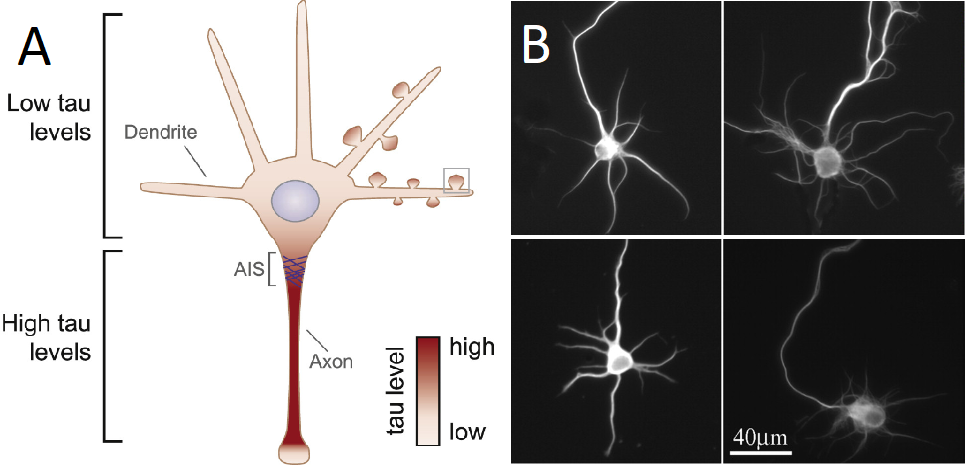
\includegraphics[width=\linewidth]{Figures/neuron.png}
	\caption[Tau in the neuronal context.]{\textbf{Tau in the neuronal context.}
	(A) Tau distribution in the neuron (adapted from \cite{Ittner2018}). Tau enrichment in the axon is facilitated by the axon initial segment (AIS) which acts as a diffusion barrier for tau. (B) Microtubule immunostains of cultured rat hippocampal neurons, adapted from \cite{Qiang2006}. Upper left: Control condition. Lower left: Depletion of tau. The panels on the right side show cells where the Katanin p60 subunit was overexpressed (with no change in tau levels in the upper panel and depletion of tau in the lower panel).
		}\label{neuron}
\end{figure}

\subsubsection{Tau}
\label{sec:tau_intro}
Tau is an intrinsically disordered protein (see \autoref{sec:proteins}) mainly found in neurons. Within the neuron, tau is mostly found in the axonal shaft, i.e. the most stable part of the neuronal microtubule architecture (\autoref{neuron}A). An important function of tau is to enhance the stability of microtubules, which it can influence directly \parencite{Drechsel1992} as well as by its capability to regulate the interaction of other MAPs with the microtubule surface \parencite{Morris2011b}. In one discovered mechanism, tau mislocalization leaves axonal microtubules unprotected against microtubule-severing enzymes, such as katanin, which leads to their destabilization and the eventual degeneration of the axon (\autoref{neuron}B) \parencite{Qiang2006}. Given the importance of microtubules, and given that tau protects microtubules, it is not surprising that malfunctions related to tau have been implicated in a number of neurodegenerative diseases \parencite{Gao2018,Morris2011b,iqbal2016tau}. For example, displacement of tau from the axon is one of the hallmark events during the onset of the Alzheimer’s disease \parencite{zempel2015tau}.  \par
As depicted in \autoref{tau}A, full-length adult tau is intrinsically disordered and includes a projection domain (its N-terminal domain), a microtubule-binding region of four imperfect sequence repeats (R1-4), and a C-terminal domain \parencite{Himmler1381}. Several different observations and explanations for how tau interacts with microtubules can be found in the literature \parencite{Morris2011b,Mcvicker2014,Kellogg2018}. For instance, it is known that tau can engage with microtubules in a mode where it diffuses along the microtubule \parencite{Hinrichs2012b}, and in another mode where it is stably bound to the microtubule \parencite{Mcvicker2014}. Recently, it was found that the tau microtubule binding repeats can bind to microtubules in a consistent, orderly fashion, enough so to allow for a high-resolution cryo-EM study (\autoref{tau}B-C) \parencite{Kellogg2018}. \par

Finally, the projection domain of tau appears to determine and cause the spacing between the microtubules within axonal microtubule arrays \parencite{Chen1992}.
\begin{figure}[h!tb]
\centering
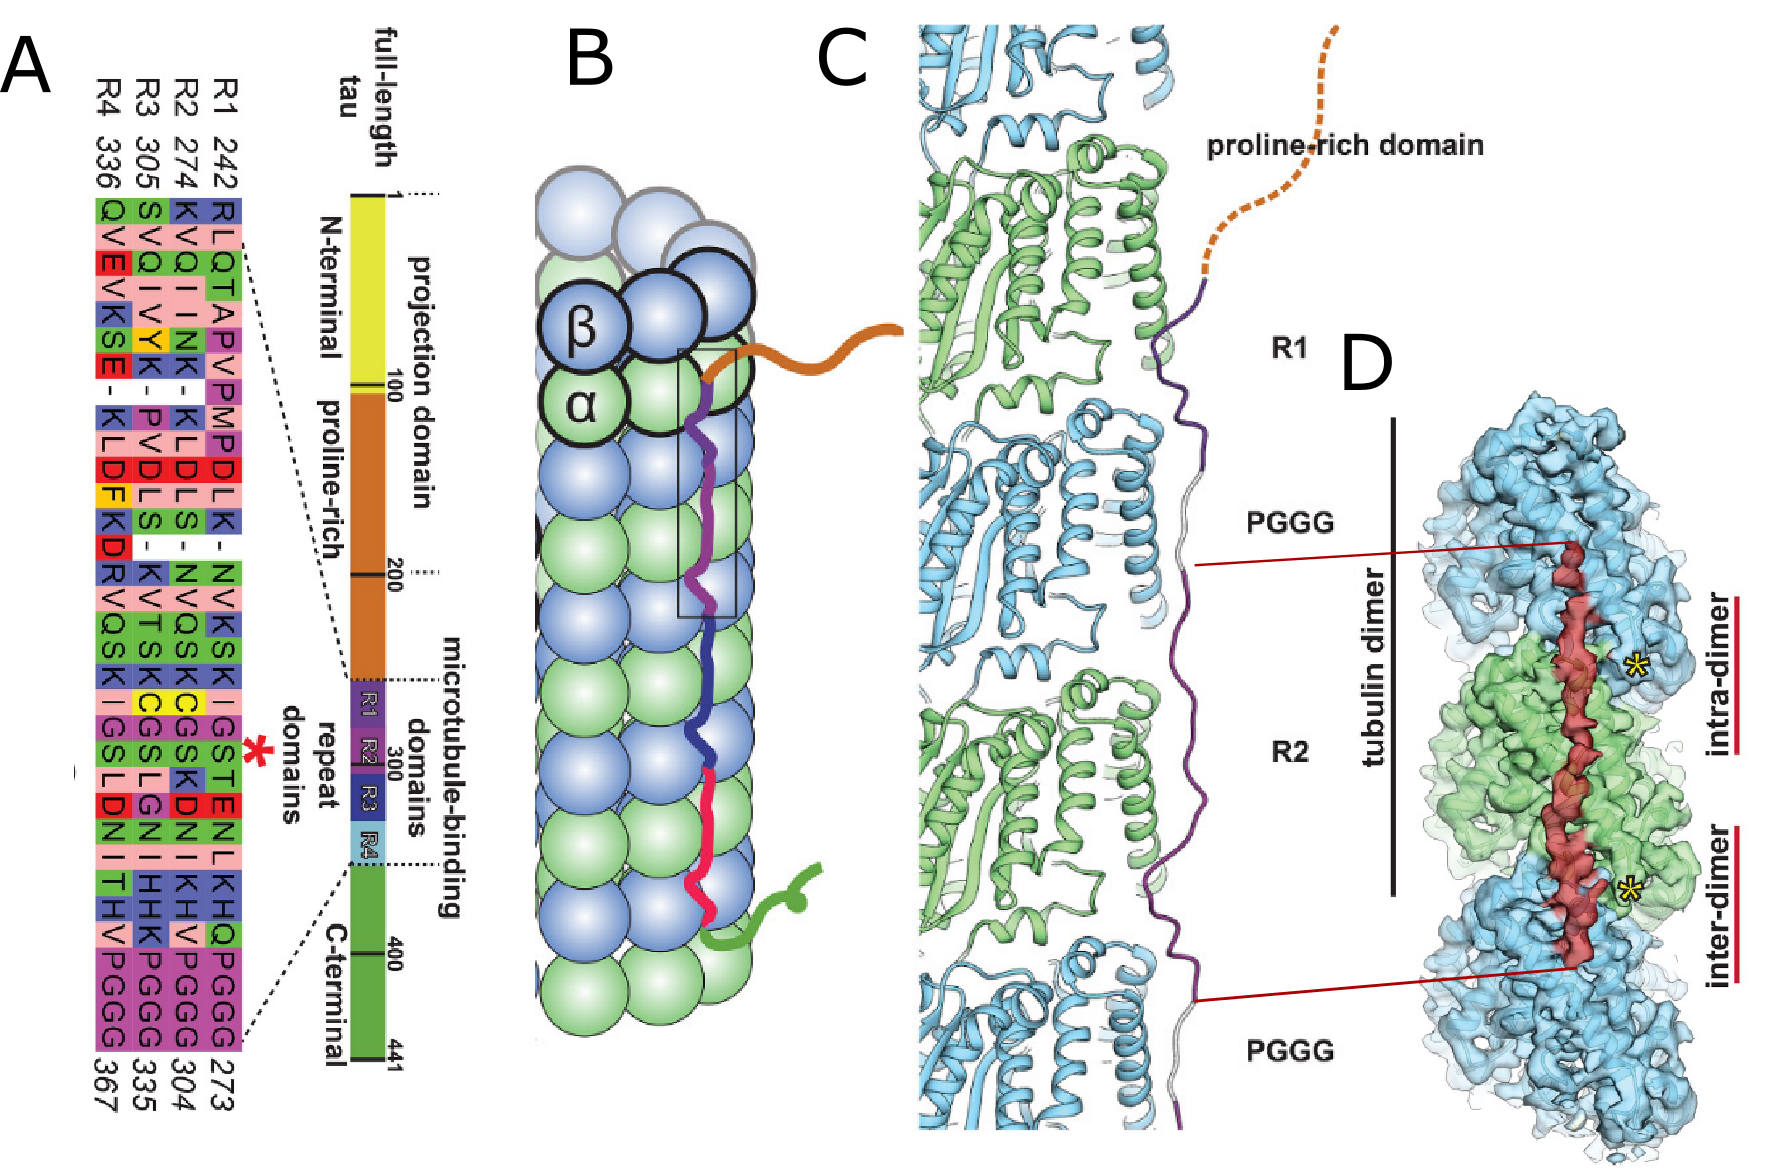
\includegraphics[width=\linewidth]{Figures/tau.png}
\caption[Introduction to tau.]{\textbf{Introduction to tau.}
(A) Schematic of the domains of tau protein. Inset shows the sequence alignment of the four microtubule binding repeat sequences, R1-4, that make up the repeat domain. (B) Model of full-length tau binding to microtubules and tubulin oligomers proposed by a recent cryo-EM study \parencite{Kellogg2018}. (C) Detailed representation of that model. (D) Cryo-EM density map of a part of the microtubule surface under the presence of tau, as observed by \cite{Kellogg2018} (top view, looking onto the surface of the microtubule). The additional density (in addition to tubulin) is colored in red and likely due to tau binding to the microtubule with its microtubule binding repeats. The PGGG sequences between the repeats were not visible on the density map, indicating that they did not bind to the microtubules in an orderly fashion. Adapted from \cite{Kellogg2018}. 
	}\label{tau}
\end{figure}

\subsubsection{Katanin}
\label{sec:katanin_intro}
Katanin is a microtubule-severing enzyme that plays a critical role in the remodeling of the microtubule cytoskeleton by generating internal breaks in microtubules. This severing function modulates microtubule dynamics and organization, contributing to essential processes such as cell division, migration, and neuronal development \parencite{ROLLMECAK201096, Lombino2019}. Katanin is a heterodimer composed of two subunits: a catalytic p60 subunit and a regulatory p80 subunit. The p60 subunit belongs to the AAA+ (ATPases Associated with various cellular Activities) protein family, containing the ATPase motor domain responsible for generating mechanical force required for microtubule severing \parencite{Johjima2015, McNally2014}. While the p60 subunit has been shown to on its own exhibit microtubule-severing activity \parencite{McNally2014}, the p80 subunit has been shown to regulate the spatial distribution of katanin by targeting katanin to the centrosome \parencite{Hartman1998}. This spatial regulation is vital, as indiscriminate severing of microtubules can lead to deleterious effects on cell function. In addition to its centrosomal localization, the p80 subunit plays a role in regulating the overall activity of the catalytic p60 subunit \parencite{McNally2000}. \par

Katanin's severing activity appears to at least partially depend on ATP hydrolysis. ATP binding and subsequent hydrolysis stimulated by the microtubule provide the energy required for conformational changes in the p60 subunit, enabling it to exert mechanical force on the microtubule lattice \parencite{Zehr2017}. Specifically, katanin is thought to pull on the C-terminal tails of tubulin subunits, destabilizing the lateral interactions between protofilaments in a step-wise manner, leading to local lattice destabilization and often microtubule breakage \pref{katanin}{}. After the microtubule breakage, whether the newly created microtubule plus end polymerizes or depolymerizes depends on the presence of free tubulin \parencite{Vemu2018, Kuo2021}. At a low free tubulin concentration, the newly-created plus end will shrink. However, if there is sufficient free tubulin present, the microtubule has a high chance of entering a growth regime, because the likelyhood is high that at the site of breakage, a sufficient number of GTP-tubulin has been incorporated, establishing a protective cap (see \autoref{sec:instability}). Similarly, it should be noted that incorporation of GTP-tublin also occurs at microtubule sites where severing is not fully completed, which can lead to the emergence of GTP islands in the lattice with higher resistance against depolymerization \parencite{Vemu2018}. These mechanisms can explain the perhaps counterintuitive phenomenon that the loss of Katanin has been found to cause a decrease in microtubule mass \parencite{Vemu2018}. 
\par
In addition to it's severing activity, Katanin also promotes depolymerization of microtubules from their ends, in a manner which is independent from ATP hydrolisis and the C-terminal tails of tubulin \parencite{Belonogov2019}.

\begin{figure}[h!tb]
\centering
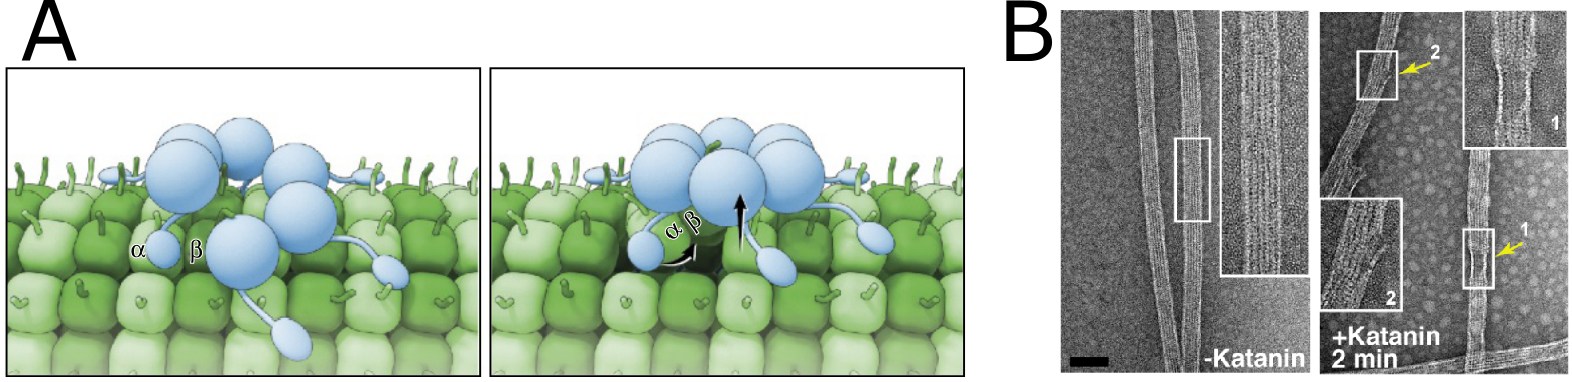
\includegraphics[width=\linewidth]{Figures/katanin.png}
\caption[Introduction to katanin.]{\textbf{Introduction to katanin.}
(A) Cartoon illustrating how katanin is hypothesized to extract tubulin dimers. Left, katanin (blue) assembles as a hexamer with each monomer's N-terminal domain emanating from the motor core and making multivalent interactions with the microtubule (green). The flexible tubulin C-terminal is engaged in the axial pore of the katanin hexamer. Right, ATP hydrolysis leads to closure of the ring that drags with it the bound C-terminal tail of a tubulin monomer. The cycle is repeated until lattice contacts unravel and the microtubule severs. Adapted from \cite{Zehr2017}. (B) GMPCPP-microtubules incubated with buffer or 100 nM katanin and visualized by transmission electron microscopy. Arrows indicate damage in the microtubule lattice. Adapted from \cite{Grigorieff2018}.
	}\label{katanin}
\end{figure}

\subsubsection{Kinesin-8/Kip3}
\label{sec:kip3_intro}
Molecular motors convert chemical energy in form of ATP into mechanical energy. One of the three large superfamilies of molecular motors are kinesins. To date more than 600 kinesin sequences with 45 kinesin genes in the human- 17 -genome \parencite{Endow3420} have been identified. Kinesins are divided into 14 kinesin sub-families based on their structure and function. I worked with Kip3, a kinesin-8 family found in budding yeast. This kinesin, like the first discovered kinesin kinesin-1 \parencite{Endow3420}, Kip3 is a homodimeric complex that moves toward the microtubule plus-end along protofilaments, propelled by its two motor domains connected by a neck linker which is essential for dimerization \parencite{Lin2020}. As in the case of kinesin-1, these two motor domains proceed along a given protofilament in a hand-over-hand manner, where the motor domains alternately bind to the microtubule with each step being 8 nm long, the same as the inter-tubulin-dimer distance \parencite{Xie2021}. This directed movement is achieved via cycles of ADP release, ATP binding, and ATP hydrolisis in each of the motor domains \parencite{Xie2021}. However, while kinesin-1 typically detaches from microtubules after a few hundred steps, Kip3 is much more processive, to a point where it usually reaches the plus end of the microtubule \parencite{Varga2009}. This processivity is attributed to the tail domain of Kip3, which can bind to microtubules \parencite{SU2011751}.\par

Due to the additional affinity for the microtubule caused by its tail domain, whenever the binding of its motor domains to the microtubule gets interrupted, Kip3 has a much higher chance to diffuse along the microtubule rather than away from the microtubule \parencite{Xie2021}. If there is no available binding site within reach, Kip3 pauses for extended periods of time \parencite{Varga2009}, resulting in the formation of traffic jams at the end of microtubules \parencite{Leduc2012}. Moreover, Kip3 has the conspicuous characteristics of being able to switch protofilaments with a leftwards bias \parencite{Bormuth2012}, and promoting microtubule depolymerization at the microtubule plus end \parencite{Lin2020}. The latter enables the cell to differentially regulate microtubule length via Kip3, as more Kip3 molecules land on longer microtubules, which therefore experience more Kip3 residence at their plus ends than short microtubules and thus a higher depolymerization activity \parencite{Varga2009}. The above points are illustrated in \autoref{kip3}.\par

Finally, the microtubule interaction sites of kinesin motor domains and the microtubule binding repeats of tau partially overlap \parencite{Kellogg2018}. Tau has been shown to regulate the microtubule interactions of the molecular motors kinesin-1 and dynein \parencite{Chaudhary2018,Dixit2008,ebneth1998overexpression,seitz2002single,trinczek1999tau,vershinin2007multiple}. However, before our study, it was unknown how tau might interact with kinesin-8. Our knowledge about kinesin-8 in neurons generally is scarce. It certainly does play an important role: A study has found that depleting Kif18A, a kinesin-8 member, increases mirotubule catastrophe frequency and reduce axon length \parencite{KEVENAAR2016849}.

\begin{figure}[h!tb]
\centering
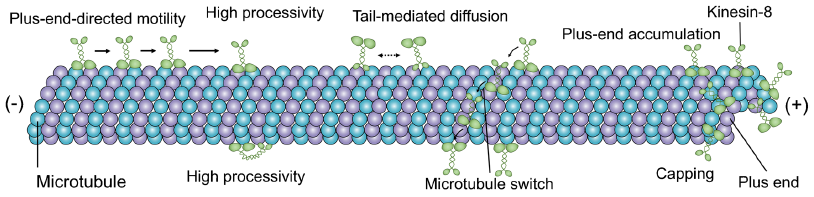
\includegraphics[width=\linewidth]{Figures/kip3.png}
\caption[Introduction to Kinesin-8/Kip3.]{\textbf{Introduction to Kinesin-8/Kip3.}
An illustration of the typical characteristics of members of the Kinesin-8 family, including Kip3. Adapted from \cite{Lin2020}.
	}\label{kip3}
\end{figure}

\subsection{The mitotic spindle}
\label{sec:spindle}
The fission yeast Schizosaccharomyces pombe (S. pombe) is a popular eukaryotic model organism for studying the cell cycle including the mitotic spindle \parencite{Vyas2021, Uzsoy2021}, in part due to its relatively low complexity, as evidenced by its small number of protein-coding genes \parencite{Wood2002}. Other than in animal cells, where the mitotic spindle is established in the cytoplasm, the mitotic spindle of S. pombe forms inside the nucleous \parencite{Kilmartin2014}. As in animals cells, the mitotic spindle allows the cell to separate its two chromosome sets (each containing the DNA for each forthcoming dauther cell) (\autoref{spindle}A).

\begin{figure}[h!tb]
	\centering
	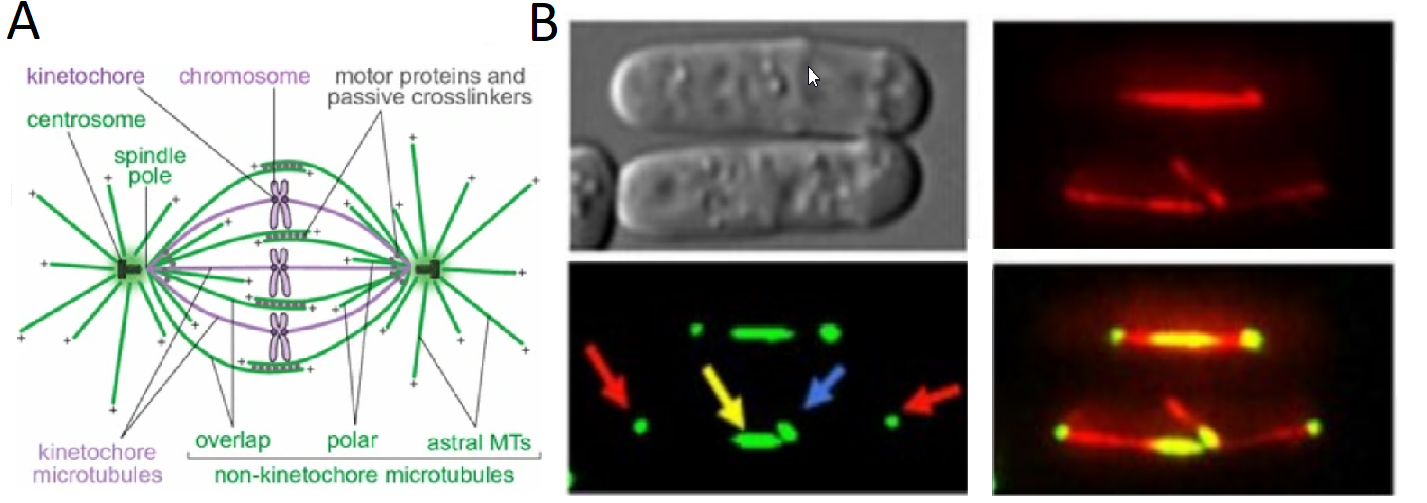
\includegraphics[width=\linewidth]{Figures/spindle.png}
	\caption[Microtubule crosslinkers in the context of the mitotic spindle.]{\textbf{Microtubule crosslinkers in the context of the mitotic spindle.}
	(A) An illustration of the mitotic spindle in animal cells (S. pombe features spindle pole bodies instead of centrosomes, and therefore no astral microtubules \parencite{Kilmartin2014}). The polar microtubules grow from the centrosome, overlapping in an antiparallel fashion in the middle of the nucleous. There, they are crosslinked by passive crosslinkers such as Ase1, but also motor proteins which together with passive crosslinkers contribute to a proper positioning of the mitotic spindle \parencite{Janson2007,Braun2011}. Adapted from \cite{Tolic2018}. The kinetochore microtubules separate the chromosomes from each other and pull them toward the centrosomes (in the next phase of mitosis not shown here). (B) 3D projection images of wild-type S. pombe cells taken during mitosis, with tubulin (CFP-tub1p) in red and Ase1 (Ase1-GFP) in green. Top-left picture taken with differential interference contrast (DIC) microscopy. The yellow arrow indicates the spindle midzone, where Ase1 is binding in between antiparallel microtubule overlaps. Adopted from \cite{Loiodice2005}.
		}\label{spindle}
\end{figure}

\subsubsection{Ase1}
\label{sec:Ase1_intro}
We were interested in the (potential) role of microtubule crosslinkers in building and maintaining the mitotic spindle, where we worked with the S. pombe protein Ase1. Ase1 is a conserved microtubule-bundling protein with orthologues e.g. in plants (MAP65) and mammals (PRC1). During mitosis, Ase1 proteins (or its orthologues in other organisms) are found preferentially at the spindle midzone (\autoref{spindle}B), and are involved in spindle integrity and regulation of spindle elongation \parencite{Loiodice2005,Yamashita2005,She2019}. S. pombe Ase1 deletion mutants, although viable, exhibit interphase microtubules with reduced bundling and mitotic spindles that often fall apart as they elongate in anaphase \parencite{Loiodice2005,Yamashita2005}. \par
Characteristically, the geometry of Ase1 favors antiparallel microtubule arrays, which results in increased Ase1/MAP65/PRC1 affinities for antiparallel microtubule overlaps and preferential antiparallel crosslinking activity \parencite{She2019,Bieling2010,Janson2007,Subramanian2010,Kellogg2016,Gaillard2008}. The preferred binding of Ase1/MAP65/PRC1 family proteins to antiparallel microtubules leads to the recruitment of other proteins that can locally alter microtubule dynamics, such as CLASP \parencite{Bratman2007b,Liu2009,Kitazawa2014} or kinesin-4 \parencite{Bieling2010, Mani2021}. By recruiting these additional factors, Ase1 family proteins can differentially regulate the dynamics of bundled microtubules, specifically affecting the dynamics of antiparallel bundles \parencite{Bieling2010,Bratman2007b, Mani2021}. Additionally, Ase1 family members themselves are also known to have direct effects on microtubule dynamics. In vitro experiments have shown that MAP65-1, upon crosslinking microtubules, promotes rescues \parencite{Stoppin-Mellet2013}. Based on the modeling of their observed overlap dynamics, \cite{Stoppin-Mellet2013} predicted MAP65-1 to have more effect on antiparallel microtubules compared to parallel ones. However, this prediction has not yet been directly experimentally validated.\par
Ase1 possesses a structured N-terminal domain, a central spectrin domain, and an intrinsically disordered C-terminal domain \parencite{Kapitein2008,Kellogg2016}. Ase1 molecules self-associate into homodimers. The N-terminal domain supports this homodimerization and is necessary for microtubule crosslinking activity \parencite{Janson2007}. The spectrin domain and the unstructured C-terminal interact with the microtubule \parencite{Kellogg2016}. Ase1 interacts with microtubules diffusively by exhibiting a one-dimensional random walk along the microtubule lattice. When diffusing on a single microtubule, the free microtubule-binding domain samples a large space, allowing for "catching" of another microtubule which subsequently is crosslinked to the first microtubule, preferably in antiparallel fashion (\cite{Janson2007}, \autoref{Ase1}). Within the resulting antiparallel microtubule bundle, Ase1 does still diffuse, albeit with an approximately eight-times lower diffusion coefficient than on single microtubules \parencite{lanskydiffusible2015}.\par
As another feature of Ase1, it has been found that microtubules decorated with Ase1 are less stiff than undecorated microtubules \parencite{Portran2013}.
\begin{figure}[h!tb]
\centering
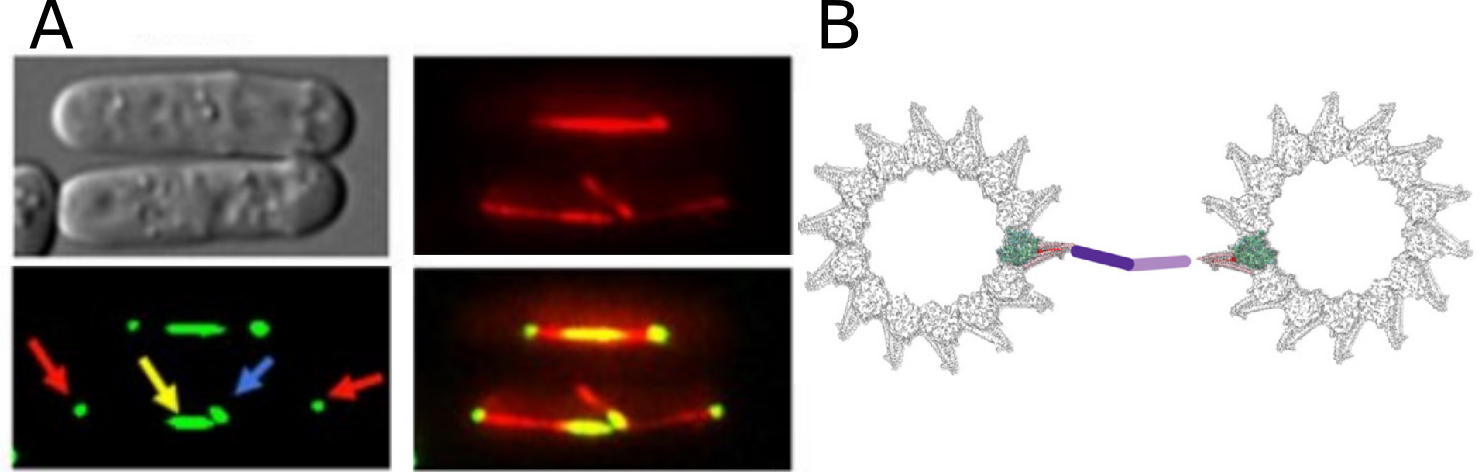
\includegraphics[width=\linewidth]{Figures/Ase1.png}
\caption[Introduction to Ase1.]{
\textbf{Introduction to Ase1.} A model of how PRC1, a Ase1 homologue, binds to two antiparallely aligned microtubules, based on cryo-EM data. The cryo-EM reconstruction is overlayed with shades of green and blue ($\alpha$ and $\beta$-tubulin) and pink (the spectrin domain, the microtubule-binding domain of PRC1 and Ase1). The dimerization domains of PRC1 are shown as cartoons in shades of purple (the cryo-EM study was conducted with a PRC1 construct without the dimerization domain). Adopted from \cite{Kellogg2016}. (A) View from side. (B) Cross section view (from bottom of what panel A shows). 
	}\label{Ase1}
\end{figure}